In order to improve the system we decided to make two experiments. The first one was aimed to found the best keyword the algorithm will recognize the most whoever is talking with whichever accent. The comprehension of the user by the algorithm is a key factor for its success. This experiment helped us to collect the best keywords each time the user have to interact with the robot. Then we experimented at the end of the development of the program a user experience to see if it was easily usable and also gives us feedback the future work. This kind of experiments can be done again in order to check the intuitiveness of each word, or to know in which order the user would like to receive the question etc. Realizing more experiments in general would have been a good plus for the project in order to adapt the more possible our program to our consumers: everyone and not only engineers.

\subsection{Confusion Matrix}
In order to prepare this experiment some instructions were prepared for both the experimenter and the user.\\
Need for the experience: 9 persons ideally with different accents.\\
Work for each user: pronounce in a normal way a list of 24 words, 3 times. Each series will be in a different order.\\
{\itshape
\\Experimenter instructions:
\begin{enumerate}
  \item Prepare the computer to record the bagfile
  \item Launch the program (\textit{roslaunch user\_experiment robot\_voice\_control.launch})
  \item Record the topic getting in the microphone (rosbag record /audio)
  \item Let the user came in the room
  \item Give the instructions to the user (see below)
  \item End the experiment by stop recording 
  \item Give explanation why this experiment is useful
\end{enumerate}

Instructions to the user (point 5)):
\begin{itemize}
  \item Say each word one by one with a pause of 2 seconds between each word
  \item Don't talk between each word
  \item Pronounce the words normally
\end{itemize}

Concerning the words tested, we selected all the words that could be use every time the user has to say something to the robot so then we can choose the ones that fit the most for each situation. Here is the list of the 24 words:
\begin{multicols}{4}
\begin{enumerate}[label=(\Alph*)]
\item teach
\item learn
\item new
\item command
\item do
\item make
\item speed
\item velocity
\item quit
\item finished
\item finish
\item end
\item yes
\item no
\item right
\item wrong
\item true
\item false
\item list
\item reset
\item restart
\item start
\item stop
\item begin 
\item other words
\end{enumerate}
\end{multicols}
}
Once we had recorded all the audio we played them all through the Pocketsphinx algorithm in order to get what the algorithm understood out of the audio recorded. So then we can compare the difference between what should be getting out and what is really getting out. This gave us the data plotted just below with the word we fixed in vertical and the results we get in horizontal: (see Figure 12)
\begin{figure}
\center
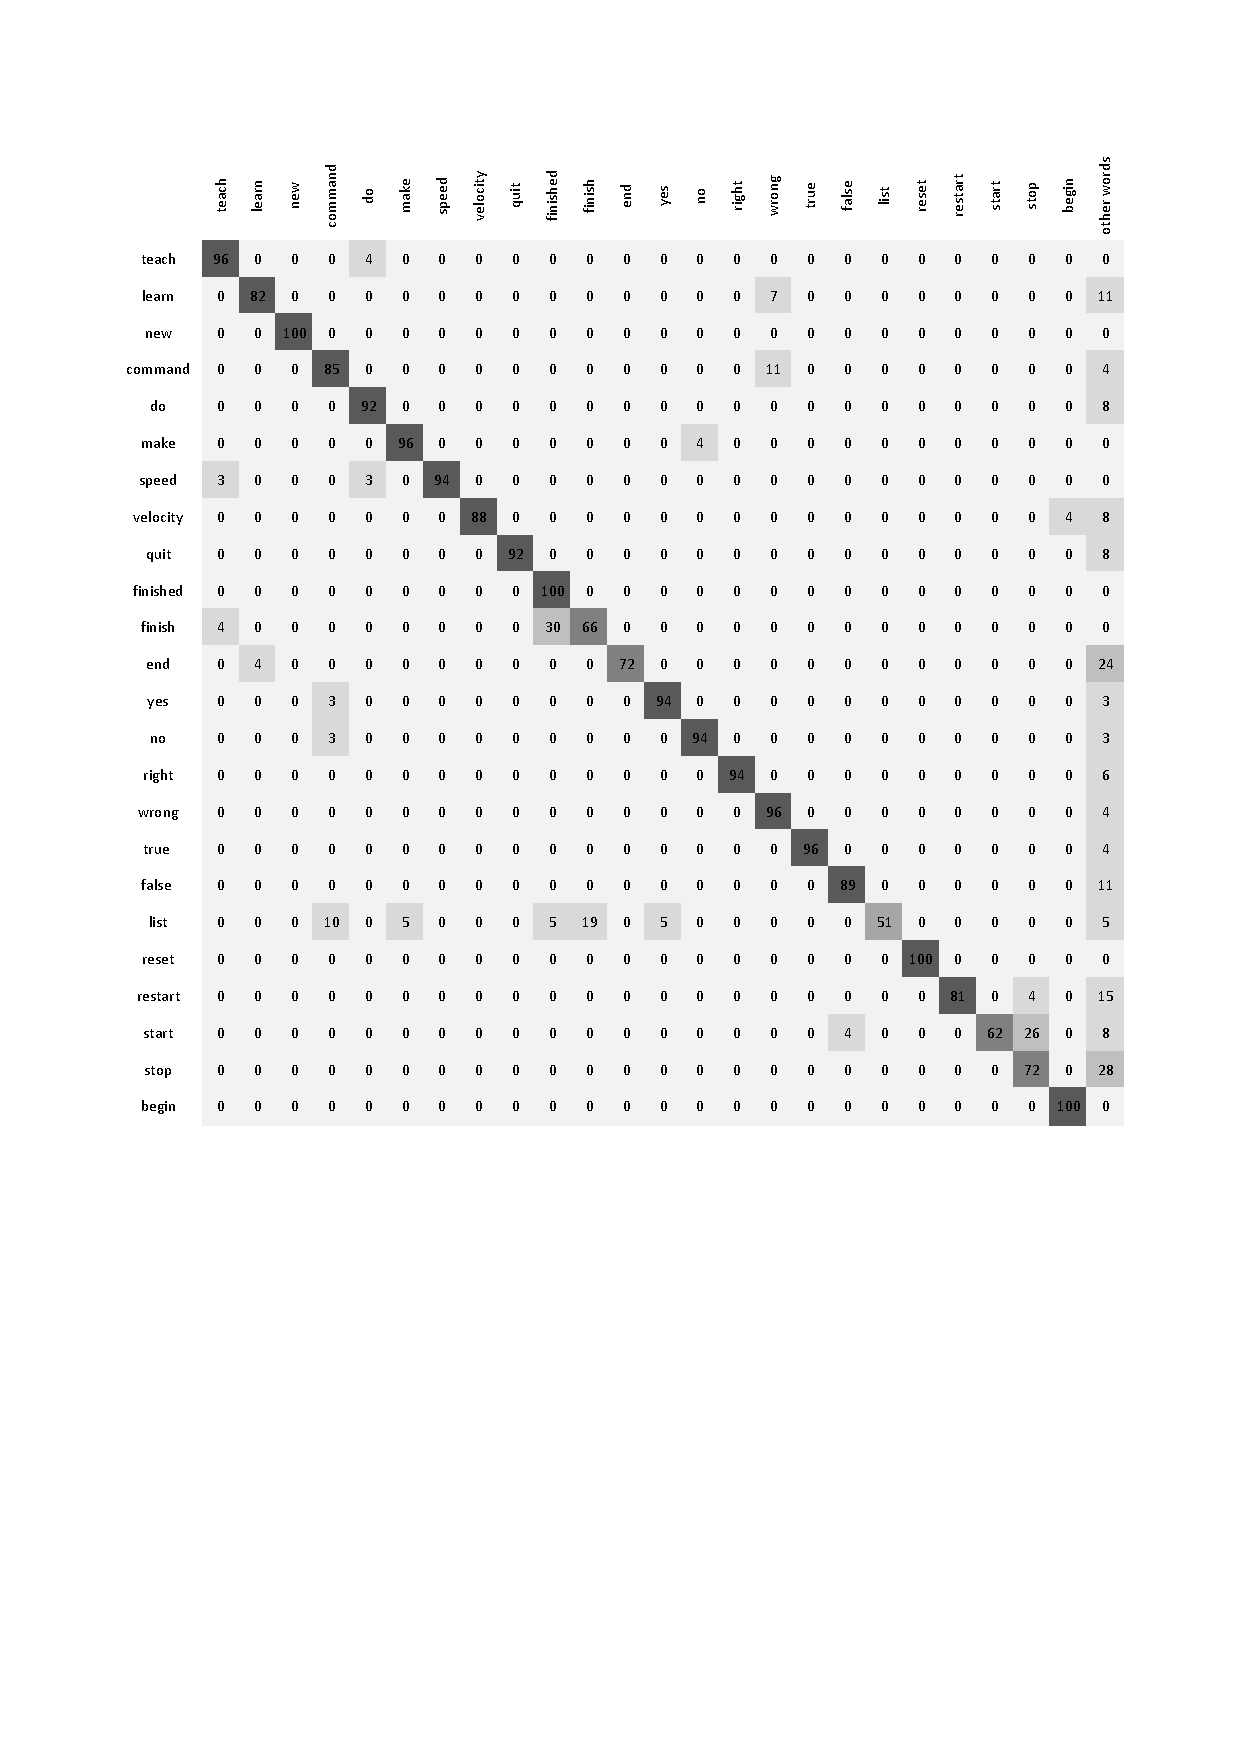
\includegraphics[width=16cm]{img/ConfusionMatrixFinal.pdf}\\
\caption{Confusion Matrix Experiment results (in percentage)}
\end{figure}

These results can let us conclude about the choice of every word for the project and here are the conclusion we made taking into consideration the results in the table and the distinctiveness of the word with all the others:
\begin{itemize}
  \item To go to the Teaching Command Machine: "Teach", "Learn" and "New"
\\We selected "Teach" and "New" since "Learn" got some confusion with some other words we cannot predict because they were in "other words".
  \item To go into the Giving Command Machine: "Command", "Do" and "Make"
\\We selected the three of them they all both got some good results. "Command" got some confusion with "Wrong", we will then remove "Wrong" from our dictionary.
  \item To go to the Changing Speed Branch: "Velocity" and "Speed"
\\We selected both words since they received some really good results.
  \item To end the program or a demonstration: "Finished", "Quit", "Finish",  "End" and "Stop"
\\We selected "Finished" and "Quit" only. The three other proposition were a lot mistaken with some other words we are using.
  \item Negation: "No", "False" and "Wrong"
\\We selected "No" and "False" since they got good results. We eliminated "Wrong" because of confusions with anterior words.
  \item Affirmation: "Yes", "Right" and "True"
\\We selected "Yes" and "True" since they got good results. We didn't select "Right" because it is the antonym of "Wrong".
  \item To access to the list of commands: "Command" and "List"
\\We selected only "Command" because "List" received some really bad results and had many confusions with words already selected.
  \item To restart: "Reset" and "Restart"
\\"Reset" got a better result than "Restart" but the results remain good so we selected both.
  \item To begin a demonstration: "Begin" and "Start"
\\We selected "Begin" and "Start". In fact in the confusion matrix we had a lot of confusion with "Stop" but we deleted it so we can assume the results will be better without "Stop".
\end{itemize}

We tried to minimize the dictionary at the maximum this is the reason we tried not put all the words with the same meaning, in fact the biggest the dictionary is, the bigger the chance a confusion between two words can be made. Minimizing the dictionary will improve the robustness of the recognition of the words said by the user.


\subsection{System Usability Scale}
The aim of this experiment was to let users who knows nothing about the project try to control the robot we developed in order to get feedback on its usability and the ways to improve. 

The user were given a paper giving the following instructions and informations:
  {\itshape
\begin{itemize}
\item Introduction:
Robot introduces itself and gives you the different opportunity you have to go through the program. It will also give you the keywords. The code will begin with an introduction and then wait in the READY STATE for you to say what you want it to do. General remark: Do not use the keyboard outside the use of teaching.

\item What you want to do? :
Once the robot introduction is done you have 4 possibilities:
\begin{itemize}
  \item Quit the program by saying the keyword � quit �
  \item Changing the speed of the branch by using the keyword � speed �
  \item Giving a command to execute to the robot by using the keyword � command � 
  \item Teach a command to the robot by using the keyword � teach �
\end{itemize}

\item Important note: 
\begin{itemize}
  \item You can reset at anytime if you are lost and want to redo it from the beginning.
  \item If the robot didn't acknowledge your saying it means that you miss-said the word: repeat yourself.
  \item You will be able to use the keyboard to teach the turtle some movements, but you won?t be able to use it any other time.
  \item Finally, every time you use the teaching branch your position will be reset at the middle of the screen. We strongly encourage you to teach everything you will need at the beginning and then try to reach the goals.
  \item When you finish the demonstration, don't forget to repeat the name of the command you are currently teaching.
\end{itemize}

\item The dictionary you have at your disposal is the following one:
Right, left, up, front, down, back, speed, � Numbers � (one to eleven), teach, start, stop, reset, velocity, wrong, right, true, false.\\


\item Experiment Explanation to the user:
\begin{enumerate}
  \item You will get 10 minutes to use the state machine and feeling comfortable with the interface.
  \item You will have to attain two goal
  	\begin{enumerate}
  	  \item The two objectives will be the following:
	  	\begin{enumerate}
		  \item First you will have to touch the right wall 
		  \item Then you will have to reach the up-left corner.
		\end{enumerate}
	\item If you are stuck and do not know what to do, you can ask for my help and I will reset the code.
	\item Every time you will teach a command to the robot, the position of the turtle will be reset.
        \end{enumerate}
  \item You will have to answer a small survey
  	\begin{enumerate}
	  \item Few questions will be asked in order to improve the project
	\end{enumerate}
\end{enumerate}

\end{itemize}
} 
For this experiment we decided to evaluate three things in addition to the completion of a System Usability Scale. The three things we evaluated were the following: 
\begin{itemize}
  \item Number of time the user required the help of the experimenter
  \item Number of time the user required information from the experimenter
  \item Number of location goals reached (the user had to reach the right border first and then the top-left corner)
\end{itemize}

Concerning the results we will analyze each user:
\begin{itemize}
  \item The first user was directly blocked at the beginning when he had to teach a command to the robot. The algorithm couldn't understand him saying "Start" to record a command. In fact during this experiment the robot had no command already taught at the beginning. Additionally to that the user felt lost once I helped him for the "Start" word because of a specificity of the code. After demonstrating the command the user wanted to teach to the robot, he had to repeat directly the name of the command he was teaching because at the beginning I didn't put a Say State at this place, again the user required my help here. Finally, instead of teaching the basics command, the user wanted to teach one command to reach each goal in one time. That wasn't the best way of doing it since the Teaching Command Machine is way longer to execute than the Giving Command Machine. Except these problems of use, the feedbacks were good. The user didn't reach the goal because of the problem with the word "Start".
  \item The second user succeeded better the experiment. The user required two times help during the experiment but reached the two goals. One of my interventions was to explain him again the problem after the demonstration and the second time was simply because he felt a bit lost since the robot didn't acknowledge something the user said. The reason is because the robot didn't understand what the user said. A simple explanation at the beginning could be to insist more on the fact that every time the user say something the user will receive a speech feedback from the robot.
\end{itemize}

Finally we fixed the problem the user encounter when teaching a command simply by adding a Say State after the demonstration which is asking the user to repeat the command he is teaching. In general the feedbacks were good and were saying that the program is easy to use and intuitive once an explanation of the program is done at the beginning by someone knowing the program.
